\documentclass[11pt,letterpaper]{article}

% Packages
\usepackage[margin=0.75in]{geometry}
\usepackage{fontspec}
\usepackage{xcolor}
\usepackage{tikz}
\usepackage{multicol}
\usepackage{enumitem}
\usepackage{setspace}
\usepackage{parskip}
\usepackage[hidelinks]{hyperref}

% Font setup
\setmainfont{ElMessiri-Regular}[
    Path = ../../assets/fonts/,
    Extension = .ttf,
    BoldFont = ElMessiri-Regular,
    BoldFeatures = {FakeBold=1.5},
    Scale=1.0
]

% Define colors
\definecolor{purple}{RGB}{138,43,226}
\definecolor{blue}{RGB}{30,144,255}
\definecolor{green}{RGB}{34,139,34}
\definecolor{red}{RGB}{220,20,60}
\definecolor{orange}{RGB}{255,140,0}
\definecolor{lightgray}{RGB}{245,245,245}
\definecolor{darkgray}{RGB}{100,100,100}

% Custom commands
\newcommand{\term}[1]{\textbf{\large\color{purple}#1}}
\newcommand{\category}[1]{\textcolor{darkgray}{\textit{\small [#1]}}}
\newcommand{\seealso}[1]{\textcolor{blue}{\textit{See also: #1}}}

% Header and footer
\usepackage{fancyhdr}
\pagestyle{fancy}
\fancyhf{}
\renewcommand{\headrulewidth}{0.4pt}
\renewcommand{\footrulewidth}{0.4pt}
\fancyhead[L]{\small\textit{Music Terms Encyclopedia}}
\fancyhead[R]{\small\textit{Beatmaking: Learn By Doing}}
\fancyfoot[C]{\small\thepage}

% Title formatting
\usepackage{titlesec}
\titleformat{\section}
  {\LARGE\bfseries\sffamily\color{purple}}
  {}
  {0em}
  {}
  [\vspace{-0.5em}\rule{\textwidth}{0.5pt}]

% Reduce spacing
\setlength{\parskip}{0.4em}
\setstretch{1.0}

% Custom definition environment
\newenvironment{termdef}[1]
  {\noindent\term{#1}\par\nopagebreak}
  {\par\vspace{0.3em}}

\begin{document}

% ============================================================================
% TITLE PAGE
% ============================================================================

\thispagestyle{empty}

\vspace*{\fill}

\begin{center}
{\Huge\bfseries\sffamily Music Terms}

\vspace{0.3cm}

{\LARGE\bfseries\sffamily Encyclopedia}

\vspace{0.5cm}

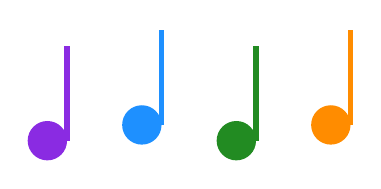
\begin{tikzpicture}
    \fill[purple] (0,0) circle (0.25cm);
    \draw[purple, line width=2pt] (0.25,0) -- (0.25,1.2);
    \fill[blue] (1.2,0.2) circle (0.25cm);
    \draw[blue, line width=2pt] (1.45,0.2) -- (1.45,1.4);
    \fill[green] (2.4,0) circle (0.25cm);
    \draw[green, line width=2pt] (2.65,0) -- (2.65,1.2);
    \fill[orange] (3.6,0.2) circle (0.25cm);
    \draw[orange, line width=2pt] (3.85,0.2) -- (3.85,1.4);
\end{tikzpicture}

\vspace{0.8cm}

{\Large\textit{Quick Reference for Music \& Production Terms}}

\vspace{0.5cm}

{\large Over 300 Essential Terms Defined}

\vspace{1cm}

\begin{center}
\fbox{\parbox{0.8\textwidth}{
\centering
\textbf{How to Use This Encyclopedia}

\vspace{0.3cm}

All terms are organized alphabetically for easy lookup. \\
Each definition is written from a beatmaker's perspective— \\
simple, clear, and practical.

\vspace{0.3cm}

\textcolor{blue}{\textit{Blue italics}} indicate related terms you can look up.
}}
\end{center}

\end{center}

\vspace*{\fill}

\begin{center}
\rule{0.8\textwidth}{0.5pt}

\vspace{0.3cm}

\textbf{Beatmaking: Learn By Doing}

\textit{www.makebeatsanywhere.com | @the\_beat\_machine\_}

\vspace{0.3cm}

\rule{0.8\textwidth}{0.5pt}
\end{center}

\newpage

% ============================================================================
% A
% ============================================================================

\section*{A}

\begin{termdef}{808}
\category{Drums}
A bass drum sound from the Roland TR-808 drum machine, famous for its deep, booming low end. The 808 kick is a staple of hip-hop, trap, and modern pop. When people say "add an 808," they usually mean a deep, sustained bass kick drum.

\seealso{Kick, Bass Drum, Sub-Bass}
\end{termdef}

\begin{termdef}{A/B Comparison}
\category{Production}
The process of switching back and forth between two versions of a mix (or between your mix and a reference track) to compare them. Helps you make better mixing decisions by hearing differences clearly.

\seealso{Reference Track, Mixing}
\end{termdef}

\begin{termdef}{Acapella (A Cappella)}
\category{General}
A vocal recording with no instrumental accompaniment. In production, acapellas are often used for remixes or to practice mixing vocals over your own beats.

\seealso{Vocals, Instrumental}
\end{termdef}

\begin{termdef}{Accent}
\category{Performance}
Emphasizing a particular note by playing it louder or with more force. Accents create dynamics and interest in your patterns—not every hit should be the same volume.

\seealso{Velocity, Dynamics, Ghost Note}
\end{termdef}

\begin{termdef}{ADSR}
\category{Sound Design}
Stands for Attack, Decay, Sustain, Release—the four stages of a sound's envelope. Controls how a sound begins (attack), fades after the initial hit (decay), holds at a steady level (sustain), and fades out when released (release). Essential for shaping synth sounds.

\seealso{Envelope, Attack, Release, Synthesizer}
\end{termdef}

\begin{termdef}{Afrobeat}
\category{Genre}
A genre originating from West Africa, characterized by complex polyrhythmic percussion, call-and-response vocals, and groovy basslines. Increasingly influential in modern pop and hip-hop production.

\seealso{Genre, Rhythm}
\end{termdef}

\begin{termdef}{Ambient}
\category{Genre}
A genre focused on atmosphere and texture rather than traditional song structure. Features sustained tones, minimal beats, and emphasis on mood. Used for background music, meditation, or cinematic production.

\seealso{Genre, Pad}
\end{termdef}

\begin{termdef}{Amplitude}
\category{Audio}
The height of a sound wave, which determines how loud it is. Higher amplitude = louder sound. Lower amplitude = quieter sound.

\seealso{Volume, Waveform, dB}
\end{termdef}

\begin{termdef}{Arp / Arpeggio / Arpeggiator}
\category{Melodic}
A chord played as a sequence of individual notes rather than all at once. An arpeggiator is a plugin that automatically creates arpeggios from the chords you play. Common in EDM, trance, and electronic music.

\seealso{Chord, Synth, Melody}
\end{termdef}

\begin{termdef}{Arrangement}
\category{Song Structure}
The organization of different sections and layers in your song—deciding what plays when, how long each section lasts, and how parts transition. Good arrangement keeps listeners engaged from start to finish.

\seealso{Song Structure, Intro, Verse, Chorus, Transition}
\end{termdef}

\begin{termdef}{Articulation}
\category{Performance}
How a note is performed—short and detached (staccato), smooth and connected (legato), accented, etc. Affects the character and feel of a melody or rhythm pattern.

\seealso{Staccato, Legato, Performance}
\end{termdef}

\begin{termdef}{Artist}
\category{Industry}
The person or group who performs or creates music. In modern production, the lines between artist, producer, and beatmaker often blur—many artists produce their own beats.

\seealso{Producer, Musician, Beatmaker}
\end{termdef}

\begin{termdef}{Attack}
\category{Sound Design / Mixing}
(1) In synthesis: How quickly a sound reaches its full volume after being triggered. Fast attack = immediate sound (drums). Slow attack = gradual fade-in (pad swells). \\
(2) In compression: How quickly the compressor responds to loud signals.

\seealso{ADSR, Envelope, Compression}
\end{termdef}

\begin{termdef}{Audio}
\category{Production}
Recorded sound (as opposed to MIDI). Audio is actual sound waves—like a recording of someone singing or a guitar being played. Once recorded, audio is "baked in" and can't be easily changed like MIDI notes.

\seealso{MIDI, Waveform, Recording}
\end{termdef}

\begin{termdef}{Audio Interface}
\category{Production}
Hardware that connects microphones, instruments, and studio monitors to your computer. Converts analog audio signals to digital (and vice versa) with better quality and lower latency than your computer's built-in sound card.

\seealso{Input, Output, Recording, Latency}
\end{termdef}

\begin{termdef}{Aux Track}
\category{Production}
See \textit{Bus}.
\end{termdef}

\newpage

% ============================================================================
% B
% ============================================================================

\section*{B}

\begin{termdef}{Backbeat}
\category{Rhythm}
The emphasis on beats 2 and 4 in a bar, typically played by the snare or clap. The backbeat is fundamental to almost all Western popular music—it's what makes you want to clap along.

\seealso{Beat, Snare, Bar, Downbeat}
\end{termdef}

\begin{termdef}{Bar / Measure}
\category{Rhythm}
A group of beats, almost always 4 beats in modern music. Songs are organized in bars: "The intro is 8 bars long" means 32 beats total. Your DAW timeline shows bar numbers.

\seealso{Beat, Time Signature, BPM}
\end{termdef}

\begin{termdef}{Bass / Bassline}
\category{Melodic}
The low-pitched musical line that provides the harmonic and rhythmic foundation of a track. The bassline usually follows the root notes of chords while also creating groove with the drums.

\seealso{Sub-Bass, Root Note, Low-End, 808}
\end{termdef}

\begin{termdef}{Bass Drum}
\category{Drums}
See \textit{Kick}.
\end{termdef}

\begin{termdef}{Bass Drop}
\category{Production}
The moment in a track (especially in EDM and dubstep) when the bass and drums hit hard after a buildup. Creates maximum impact and energy.

\seealso{Drop, Buildup, Sub-Bass}
\end{termdef}

\begin{termdef}{Bass Synth}
\category{Melodic}
A synthesizer sound designed for low-end bass. Can range from smooth sine waves to aggressive, distorted sounds. Essential for electronic music production.

\seealso{Synthesizer, Bass, Sub-Bass}
\end{termdef}

\begin{termdef}{Beat}
\category{Rhythm}
(1) The steady pulse of music—the thing you nod your head to. \\
(2) Slang for an instrumental track, especially in hip-hop: "I made a new beat."

\seealso{BPM, Rhythm, Downbeat, Instrumental}
\end{termdef}

\begin{termdef}{Beatmaker}
\category{Industry}
Someone who creates instrumental tracks (beats), especially in hip-hop and electronic music. Similar to a producer, but often focuses specifically on creating the core instrumental.

\seealso{Producer, Artist, Instrumental}
\end{termdef}

\begin{termdef}{Bit Depth}
\category{Production}
Determines the dynamic range and quality of digital audio. Common bit depths: 16-bit (CD quality), 24-bit (professional recording), 32-bit (floating point for mixing). Higher bit depth = more detail and quieter noise floor.

\seealso{Sample Rate, Audio, Recording}
\end{termdef}

\begin{termdef}{Blues}
\category{Genre}
An American music genre characterized by specific chord progressions (often I-IV-V), expressive vocals, and emotional depth. Heavily influential on rock, jazz, R\&B, and modern popular music.

\seealso{Genre, Chord Progression}
\end{termdef}

\begin{termdef}{Boom Bap}
\category{Genre}
A style of hip-hop characterized by hard-hitting kick drums and snappy snares, often with jazz or soul samples. Classic 90s East Coast hip-hop sound.

\seealso{Hip-Hop, Genre, East Coast}
\end{termdef}

\begin{termdef}{Bounce}
\category{Production}
See \textit{Export}.
\end{termdef}

\begin{termdef}{BPM (Beats Per Minute)}
\category{Rhythm}
The speed of a song, measured in beats per minute. Slow songs: 60-90 BPM. Medium: 90-120 BPM. Fast: 120-180+ BPM. Sets the energy and feel of your entire track.

\seealso{Tempo, Beat, Metronome}
\end{termdef}

\begin{termdef}{Brass}
\category{Melodic}
Instruments like trumpets, trombones, and saxophones (technically a woodwind but often grouped with brass). Add power, energy, and character to arrangements. Common in funk, jazz, and orchestral production.

\seealso{Strings, Melodic Instruments}
\end{termdef}

\begin{termdef}{Break / Breakdown}
\category{Song Structure}
A section where most elements drop out, leaving only a few layers (often just drums or just chords). Creates contrast and gives the listener a moment to breathe before building back up.

\seealso{Drop, Buildup, Arrangement}
\end{termdef}

\begin{termdef}{Breakbeat}
\category{Drums / Genre}
(1) A drum pattern that "breaks" from the standard beat, often featuring syncopation and interesting rhythms. \\
(2) A genre of electronic music built around these drum patterns, typically 130-150 BPM.

\seealso{Drum Pattern, Genre, Syncopation}
\end{termdef}

\begin{termdef}{Bridge}
\category{Song Structure}
A contrasting section that appears later in a song, typically after the second chorus. Provides variety and leads into the final chorus or outro. Usually different harmonically and melodically from verse and chorus.

\seealso{Song Structure, Verse, Chorus, Arrangement}
\end{termdef}

\begin{termdef}{Buildup / Build}
\category{Song Structure}
A section designed to create tension and anticipation before a drop or chorus. Often features rising pitch, increasing volume, filter sweeps, and drum fills.

\seealso{Drop, Tension, Song Structure}
\end{termdef}

\begin{termdef}{Buffer Size}
\category{Production}
Determines how much audio your computer processes at once. Smaller buffer = lower latency (better for recording/playing). Larger buffer = more processing power (better for mixing). Measured in samples.

\seealso{Latency, DAW, Recording}
\end{termdef}

\begin{termdef}{Bus / Aux Track}
\category{Production}
A track that combines signals from multiple other tracks. Used for group processing (like adding reverb to all drums) or creating submixes (combining all drums before they hit the master).

\seealso{Send, Master, Mixer, Insert Effect}
\end{termdef}

\newpage

% ============================================================================
% C
% ============================================================================

\section*{C}

\begin{termdef}{Cadence}
\category{Harmony}
The harmonic "punctuation" at the end of a musical phrase—how chords resolve or conclude. Think of it like a period or comma in a sentence. Creates a sense of ending or continuation.

\seealso{Chord Progression, Resolution, Harmony}
\end{termdef}

\begin{termdef}{Call and Response}
\category{Composition}
A musical conversation where one phrase (the "call") is answered by another phrase (the "response"). Common in blues, jazz, funk, and many African musical traditions. Creates engaging back-and-forth dynamics.

\seealso{Composition, Melody, Arrangement}
\end{termdef}

\begin{termdef}{Channel}
\category{Production}
In a DAW, each track or mixer strip is often called a channel. Channels hold sounds and have individual volume, pan, and effects controls.

\seealso{Track, Mixer, DAW}
\end{termdef}

\begin{termdef}{Chord}
\category{Harmony}
Three or more notes played together. Chords create the harmonic foundation of your track and set the emotional mood. Major chords sound happy; minor chords sound sad.

\seealso{Triad, Harmony, Chord Progression, Major, Minor}
\end{termdef}

\begin{termdef}{Chord Progression}
\category{Harmony}
A sequence of chords played in order, usually repeating. The harmonic backbone of most songs. Famous progressions include I-V-vi-IV (pop) and i-iv (hip-hop vamp).

\seealso{Chord, Harmony, Roman Numerals, Key}
\end{termdef}

\begin{termdef}{Chorus}
\category{Song Structure}
The main section of a song, usually the most memorable and emotionally impactful part. Contains the main hook and typically repeats multiple times. The part everyone sings along to.

\seealso{Hook, Verse, Song Structure, Bridge}
\end{termdef}

\begin{termdef}{Chorus (Effect)}
\category{Effects}
An audio effect that makes one sound like multiple sounds playing slightly out of tune and time with each other. Creates thickness and movement. Common on synths and guitars.

\seealso{Flanger, Phaser, Effects}
\end{termdef}

\begin{termdef}{Chromatic Scale}
\category{Scale}
All 12 notes in Western music: C, C\#, D, D\#, E, F, F\#, G, G\#, A, A\#, B. Moving by semitones (half-steps). Includes every possible note within an octave.

\seealso{Scale, Semitone, Octave}
\end{termdef}

\begin{termdef}{Clap}
\category{Drums}
A percussive hand-clap sound, often used instead of or alongside snare drums. Common in pop, hip-hop, and EDM. Usually hits on beats 2 and 4 (the backbeat).

\seealso{Snare, Backbeat, Drums}
\end{termdef}

\begin{termdef}{Clef}
\category{Theory}
A symbol in written music notation that tells you which notes correspond to which lines. (Treble clef for high notes, bass clef for low notes.) Not essential for beatmakers working in DAWs.

\seealso{Notation, Staff}
\end{termdef}

\begin{termdef}{Click Track}
\category{Rhythm}
See \textit{Metronome}.
\end{termdef}

\begin{termdef}{Clip / Region}
\category{Production}
A segment of audio or MIDI in your DAW timeline. You can move, copy, trim, and arrange clips to build your song.

\seealso{DAW, Timeline, Audio, MIDI}
\end{termdef}

\begin{termdef}{Clipping}
\category{Mixing}
Distortion that occurs when a signal is too loud for the system to handle. The waveform "clips" or flattens at the top, causing harsh, unpleasant distortion. Avoid clipping in your mix (unless used intentionally for effect).

\seealso{Distortion, Headroom, Limiter}
\end{termdef}

\begin{termdef}{Closed Hi-Hat}
\category{Drums}
A hi-hat cymbal hit where the two cymbals are pressed together, creating a short, tight "tss" sound. Provides rhythmic subdivision and drive. Often plays steady 8th or 16th notes.

\seealso{Hi-Hat, Open Hi-Hat, Drums}
\end{termdef}

\begin{termdef}{Collab / Collaboration}
\category{Industry}
When two or more artists, producers, or musicians work together on a track. Collaborations combine different skills, styles, and audiences.

\seealso{Feature, Producer, Artist}
\end{termdef}

\begin{termdef}{Composition / Composing}
\category{General}
The act of creating music—writing melodies, harmonies, rhythms, and arranging them into a complete piece. Composers create the musical ideas; producers shape how those ideas sound.

\seealso{Songwriting, Production, Arrangement}
\end{termdef}

\begin{termdef}{Compression / Compressor}
\category{Mixing}
An effect that reduces the dynamic range of audio by making loud parts quieter and (often) boosting the overall level. Makes mixes sound tighter, more controlled, and more "glued together." Essential mixing tool.

\seealso{Threshold, Ratio, Attack, Release, Limiter, Sidechain}
\end{termdef}

\begin{termdef}{Connector Note / Passing Tone}
\category{Theory / Composition}
A note that smoothly connects two other notes (usually chord tones). Not part of the underlying chord but creates melodic flow. Example: in Still D.R.E., the bass uses B and G as connector notes between A and E.

\seealso{Bass, Melody, Chord}
\end{termdef}

\begin{termdef}{Consonance}
\category{Harmony}
Notes or chords that sound pleasant, stable, and resolved when played together. The opposite of dissonance. Examples: octaves, perfect 5ths, major and minor triads.

\seealso{Dissonance, Harmony, Chord, Interval}
\end{termdef}

\begin{termdef}{Copyright}
\category{Industry}
Legal protection for original musical works. When you create music, you automatically own the copyright (in most countries). Copyright determines who can use, distribute, and profit from music.

\seealso{Royalties, Publishing, Industry}
\end{termdef}

\begin{termdef}{Counterpoint}
\category{Theory}
The technique of combining two or more independent melodic lines that work harmonically together. Common in classical music and jazz; less emphasized in modern beatmaking.

\seealso{Harmony, Melody, Polyphonic}
\end{termdef}

\begin{termdef}{Country}
\category{Genre}
An American genre characterized by storytelling lyrics, acoustic instruments (guitar, fiddle), and often simple chord progressions. Influence modern pop and has sub-genres ranging from traditional to pop-country.

\seealso{Genre}
\end{termdef}

\begin{termdef}{Cowbell}
\category{Drums}
A metallic percussion instrument with a distinct "tonk" sound. Famous from the "More Cowbell" SNL sketch. Used for accents and to add character to drum patterns.

\seealso{Percussion, Drums}
\end{termdef}

\begin{termdef}{Crash (Cymbal)}
\category{Drums}
A large cymbal that creates a loud, explosive "crash" sound. Used for emphasis at the beginning of sections, for climactic moments, or to mark transitions.

\seealso{Ride, Drums, Percussion}
\end{termdef}

\begin{termdef}{Cutoff (Filter)}
\category{Sound Design}
The frequency at which a filter begins to cut (remove) frequencies. In a low-pass filter, the cutoff determines how much high-end is removed. Moving the cutoff creates the classic "wah" or sweeping sound.

\seealso{Filter, Low-Pass Filter, High-Pass Filter, Resonance}
\end{termdef}

\newpage

% ============================================================================
% D
% ============================================================================

\section*{D}

\begin{termdef}{DAW (Digital Audio Workstation)}
\category{Production}
Software for recording, editing, mixing, and producing music. Examples: Ableton Live, FL Studio, Logic Pro, Pro Tools. Your DAW is your complete music production studio on a computer.

\seealso{Production, MIDI, Audio, Mixing}
\end{termdef}

\begin{termdef}{dB (Decibel)}
\category{Audio}
The unit for measuring audio levels. 0 dB is the maximum level before clipping in digital audio. Negative dB values (-6 dB, -12 dB) indicate quieter levels. Each 6 dB represents roughly a doubling or halving of volume.

\seealso{Volume, Amplitude, Clipping}
\end{termdef}

\begin{termdef}{Deep House}
\category{Genre}
A subgenre of house music with emphasis on atmosphere, chord progressions, and soulful elements. Typically 120-125 BPM with smooth, groovy basslines and lush pads.

\seealso{House, EDM, Genre}
\end{termdef}

\begin{termdef}{Degree (Scale Degree)}
\category{Theory}
A note's position within a scale, numbered 1-7 (or 1-8 including the octave). In C Major: C=1st degree, D=2nd, E=3rd, etc. Helps understand chord and melody construction.

\seealso{Scale, Root Note, Key}
\end{termdef}

\begin{termdef}{Delay}
\category{Effects}
An effect that repeats a sound after a set amount of time. Creates echoes. Can be short (slapback delay) or long (atmospheric echoes). Essential for adding space and movement to sounds.

\seealso{Echo, Reverb, Effects}
\end{termdef}

\begin{termdef}{Demo}
\category{Industry}
A rough or preliminary version of a song, used to demonstrate ideas. Demos are often sent to collaborators, record labels, or used as reference before creating the final version.

\seealso{Rough Mix, Production}
\end{termdef}

\begin{termdef}{Diatonic}
\category{Theory}
Notes or chords that belong to a particular key or scale. If you're in C Major, all the notes from the C Major scale are diatonic. Notes outside the scale are non-diatonic (chromatic).

\seealso{Key, Scale, Chromatic}
\end{termdef}

\begin{termdef}{Distortion}
\category{Effects}
An effect that adds grit, edge, and harmonic richness by clipping or overdriving the audio signal. Ranges from subtle warmth to aggressive crunch. Common on guitars, bass, and drums.

\seealso{Saturation, Clipping, Effects}
\end{termdef}

\begin{termdef}{Distribution}
\category{Industry}
The process of getting your music onto streaming platforms (Spotify, Apple Music, etc.) and digital stores. Distribution services handle this for independent artists.

\seealso{Release, Streaming, Industry}
\end{termdef}

\begin{termdef}{Dominant 7th}
\category{Harmony}
A type of 7th chord built on the 5th degree of a scale, with a strong pull back to the tonic (home) chord. Creates tension that wants to resolve. Notation example: G7 in the key of C Major.

\seealso{7th Chord, Chord, Resolution, Tension}
\end{termdef}

\begin{termdef}{Downbeat}
\category{Rhythm}
The first beat of a bar—beat 1. The strongest, most emphasized beat. When you count "1, 2, 3, 4," the "1" is the downbeat.

\seealso{Beat, Upbeat, Bar, Backbeat}
\end{termdef}

\begin{termdef}{Downtempo}
\category{Genre}
Electronic music with a slower tempo (typically 70-110 BPM) and emphasis on atmosphere and groove rather than energy. Often chill and introspective.

\seealso{Genre, Ambient, Trip-Hop}
\end{termdef}

\begin{termdef}{Drop}
\category{Song Structure}
The moment of maximum impact in a song, especially in EDM. After a buildup, the drop brings in the full beat, bass, and energy. The "payoff" moment that makes crowds go wild.

\seealso{Buildup, Bass Drop, Song Structure}
\end{termdef}

\begin{termdef}{Dry Signal}
\category{Mixing}
Audio without any effects applied. The "dry" version is the original, unprocessed sound. Often blended with the "wet" (effected) signal.

\seealso{Wet Signal, Effects, Mixing}
\end{termdef}

\begin{termdef}{Drum \& Bass / DnB}
\category{Genre}
A high-energy electronic genre characterized by fast breakbeats (160-180 BPM) and heavy sub-bass. Originated in the UK in the 1990s.

\seealso{Genre, Breakbeat, Sub-Bass}
\end{termdef}

\begin{termdef}{Drum Fill}
\category{Drums}
A short, decorative drum pattern that "fills" space between sections. Often used to signal a transition (from verse to chorus). Adds excitement and variation.

\seealso{Drums, Transition, Tom}
\end{termdef}

\begin{termdef}{Drum Kit / Drum Set}
\category{Drums}
A collection of drums and cymbals played together: kick, snare, hi-hat, toms, and cymbals. In production, this refers to the complete set of drum sounds you use in a track.

\seealso{Kick, Snare, Hi-Hat, Tom, Crash}
\end{termdef}

\begin{termdef}{Drum Loop}
\category{Drums}
A repeating drum pattern. Can be a pre-recorded audio loop or a MIDI pattern you've programmed. The rhythmic foundation that repeats throughout a section.

\seealso{Loop, Drums, Beat}
\end{termdef}

\begin{termdef}{Drum Pattern}
\category{Drums}
The specific arrangement of drum hits—which drums hit on which beats. Every genre has characteristic drum patterns (e.g., four-on-the-floor for house, boom-bap for hip-hop).

\seealso{Drums, Beat, Groove, Pattern}
\end{termdef}

\begin{termdef}{Dubstep}
\category{Genre}
Electronic genre characterized by heavy sub-bass, syncopated rhythms, and aggressive "wobble" bass sounds. Typically around 140 BPM but feels half as fast due to the rhythm structure.

\seealso{Genre, EDM, Sub-Bass}
\end{termdef}

\begin{termdef}{Ducking}
\category{Mixing}
When one sound automatically gets quieter to make room for another sound. Often achieved with sidechain compression. Example: music ducking under a podcast voice.

\seealso{Sidechain, Compression, Mixing}
\end{termdef}

\begin{termdef}{Dyad}
\category{Harmony}
Two notes played together. Simpler than a full chord but still creates harmony. Power chords (root + 5th) and the Still D.R.E. piano riff (C + A) are dyads.

\seealso{Chord, Interval, Harmony}
\end{termdef}

\begin{termdef}{Dynamics}
\category{Performance / Mixing}
The variation between loud and quiet in music. Good dynamics create interest and emotion. In mixing, dynamics refer to tools like compression that control volume changes.

\seealso{Velocity, Compression, Volume}
\end{termdef}

% ============================================================================
% E
% ============================================================================

\section*{E}

\begin{termdef}{East Coast (Hip-Hop)}
\category{Genre}
A style of hip-hop that originated in New York and the eastern United States. Characterized by complex lyricism, jazz/soul samples, and boom-bap production. Artists: Wu-Tang Clan, Nas, Jay-Z.

\seealso{Hip-Hop, Boom Bap, West Coast}
\end{termdef}

\begin{termdef}{Echo}
\category{Effects}
A distinct repetition of a sound, similar to delay but often refers to longer, more pronounced repetitions. The difference between echo and delay is subtle—echo suggests a more natural, spacious repetition.

\seealso{Delay, Reverb, Effects}
\end{termdef}

\begin{termdef}{EDM (Electronic Dance Music)}
\category{Genre}
Umbrella term for electronic music made for dancing. Includes house, techno, dubstep, trance, drum \& bass, and many other subgenres. Characterized by strong beats, synthesized sounds, and buildups/drops.

\seealso{House, Techno, Dubstep, Genre}
\end{termdef}

\begin{termdef}{Effect Plugin}
\category{Production}
A plugin that processes audio (as opposed to generating it). Examples: EQ, compression, reverb, delay. Effects shape and enhance sounds but don't create them.

\seealso{Plugin, Insert Effect, Send, Instrument Plugin}
\end{termdef}

\begin{termdef}{Electro}
\category{Genre}
Electronic music style characterized by drum machines (especially the 808), vocoders, and robotic sounds. Influential in the development of hip-hop, techno, and modern electronic music.

\seealso{Genre, 808, EDM}
\end{termdef}

\begin{termdef}{Engineer / Sound Engineer}
\category{Industry}
A technical specialist who operates recording equipment, sets up sessions, and ensures proper audio quality. Often distinct from the producer, though roles can overlap.

\seealso{Mix Engineer, Mastering Engineer, Producer}
\end{termdef}

\begin{termdef}{Envelope}
\category{Sound Design}
The shape of a sound over time—how it starts, sustains, and ends. Described by ADSR: Attack (how it starts), Decay (initial fade), Sustain (held level), Release (how it ends).

\seealso{ADSR, Attack, Release, Sound Design}
\end{termdef}

\begin{termdef}{EQ / Equalization}
\category{Mixing}
The process of adjusting the balance of frequencies in audio. Boost bass, cut harsh highs, enhance mids—EQ is the most fundamental mixing tool. Every mix engineer uses EQ on almost every track.

\seealso{High-Pass Filter, Low-Pass Filter, Frequency, Mixing}
\end{termdef}

\begin{termdef}{Export / Bounce / Render}
\category{Production}
Converting your DAW project into a final audio file (WAV, MP3, etc.). Exports freeze all your MIDI, plugins, and effects into a stereo mix you can share or upload.

\seealso{Mix Down, Two-Track, Master, DAW}
\end{termdef}

\begin{termdef}{Expression}
\category{Performance}
The emotional or dynamic quality brought to a performance. In MIDI, expression can be controlled through velocity, modulation, pitch bend, and other parameters.

\seealso{Velocity, Dynamics, Performance}
\end{termdef}

\newpage

% ============================================================================
% F
% ============================================================================

\section*{F}

\begin{termdef}{Fader}
\category{Mixing}
A slider control (physical or digital) that adjusts volume. In your DAW mixer, each track has a fader. Moving it up = louder, down = quieter.

\seealso{Volume, Mixer, Level}
\end{termdef}

\begin{termdef}{Feature / Featuring}
\category{Industry}
When an artist appears on another artist's track. Notation: "Artist A ft. Artist B" or "Artist A feat. Artist B."

\seealso{Collaboration, Artist}
\end{termdef}

\begin{termdef}{Feel}
\category{Performance}
The subjective quality of timing, groove, and expression in music. Two drummers can play the same pattern with different "feel"—one might be laid back, another might push ahead.

\seealso{Groove, Timing, Pocket, Swing}
\end{termdef}

\begin{termdef}{Filter}
\category{Sound Design}
A processor that removes or emphasizes certain frequencies. Low-pass filters remove highs. High-pass filters remove lows. Filters are essential for shaping synth sounds and cleaning up mixes.

\seealso{Cutoff, Resonance, EQ, Low-Pass Filter, High-Pass Filter}
\end{termdef}

\begin{termdef}{Final Mix}
\category{Production}
The completed, polished version of a song ready for mastering. All levels, EQ, effects, and arrangement decisions are finalized.

\seealso{Mixing, Master, Rough Mix}
\end{termdef}

\begin{termdef}{Flanger}
\category{Effects}
An effect that creates a "whooshing" or "jet plane" sound by mixing a signal with a delayed copy of itself. The delay time is modulated, creating a distinctive sweeping effect.

\seealso{Phaser, Chorus, Effects}
\end{termdef}

\begin{termdef}{Flat (♭)}
\category{Pitch}
Lowering a note by one semitone (half-step). B♭ is one semitone lower than B. The opposite of sharp.

\seealso{Sharp, Semitone, Natural}
\end{termdef}

\begin{termdef}{Floor Tom}
\category{Drums}
The largest tom drum, with the deepest pitch. Usually positioned on the floor (hence the name). Used for fills and low melodic drum hits.

\seealso{Tom, Drums}
\end{termdef}

\begin{termdef}{Four-on-the-Floor}
\category{Rhythm}
A drum pattern where the kick hits on every beat (1, 2, 3, 4). Fundamental to house, techno, disco, and most dance music. Creates driving, relentless energy.

\seealso{Kick, House, EDM, Drum Pattern}
\end{termdef}

\begin{termdef}{Frequency}
\category{Audio}
The rate at which a sound wave vibrates, measured in Hertz (Hz). Low frequencies = bass. High frequencies = treble. Human hearing: roughly 20 Hz to 20,000 Hz (20 kHz).

\seealso{Hz, Pitch, EQ}
\end{termdef}

\begin{termdef}{Funk}
\category{Genre}
An American genre emphasizing groove, syncopated rhythms, and strong bass. Highly influential on hip-hop, R\&B, and modern production. Artists: James Brown, Parliament-Funkadelic, Sly \& the Family Stone.

\seealso{Genre, Groove, Syncopation}
\end{termdef}

\begin{termdef}{Future Bass}
\category{Genre}
A modern EDM subgenre featuring bright synths, chopped vocals, lush chords, and energetic drops. Popular in the 2010s. Artists: Flume, Illenium, San Holo.

\seealso{EDM, Genre, Bass}
\end{termdef}

\newpage

% ============================================================================
% G
% ============================================================================

\section*{G}

\begin{termdef}{Gain}
\category{Mixing}
See \textit{Volume}.
\end{termdef}

\begin{termdef}{Genre}
\category{General}
A category or style of music characterized by specific sounds, rhythms, and production techniques. Understanding genres helps you know what production choices to make. Examples: Hip-hop, House, Rock, Jazz.

\seealso{Hip-Hop, EDM, House, Trap}
\end{termdef}

\begin{termdef}{G-Funk}
\category{Genre}
A style of West Coast hip-hop pioneered by Dr. Dre in the early 1990s. Features melodic synthesizers, heavy bass, laid-back grooves, and often uses funk samples. "Still D.R.E." is a classic G-Funk track.

\seealso{Hip-Hop, West Coast, Funk}
\end{termdef}

\begin{termdef}{Ghost Note}
\category{Performance}
A very quiet note, barely audible but felt. Ghost notes add groove and texture without dominating the mix. Essential in funk, jazz, and hip-hop drum patterns.

\seealso{Velocity, Accent, Drums, Groove}
\end{termdef}

\begin{termdef}{Glide}
\category{Sound Design}
See \textit{Portamento}.
\end{termdef}

\begin{termdef}{Grid}
\category{Production}
The vertical lines in your DAW that divide time into beats and subdivisions. Helps you place notes precisely on the timeline. Can be set to quarter notes, 8th notes, 16th notes, etc.

\seealso{Quantize, Beat, DAW, Timeline}
\end{termdef}

\begin{termdef}{Groove}
\category{Performance}
The feel and rhythmic character of music—the thing that makes you move. Groove is a combination of timing, swing, accents, and pocket. Good groove is what separates mechanical beats from musical ones.

\seealso{Feel, Pocket, Swing, Rhythm}
\end{termdef}

\begin{termdef}{Guitar}
\category{Melodic}
A stringed instrument played by strumming or plucking. Can play chords, melodies, or bass lines. Common in rock, pop, blues, and increasingly used as samples in hip-hop and electronic music.

\seealso{Bass, Melodic Instruments}
\end{termdef}

\newpage

% ============================================================================
% H
% ============================================================================

\section*{H}

\begin{termdef}{Half Note}
\category{Rhythm}
A note that lasts 2 beats in 4/4 time. Twice as long as a quarter note, half as long as a whole note.

\seealso{Quarter Note, Whole Note, Time Signature}
\end{termdef}

\begin{termdef}{Half-Step}
\category{Pitch}
See \textit{Semitone}.
\end{termdef}

\begin{termdef}{Hard Hit}
\category{Performance}
Playing a note with maximum or near-maximum velocity. Creates emphasis and power. The opposite of a soft hit.

\seealso{Velocity, Accent, Soft Hit}
\end{termdef}

\begin{termdef}{Harmony}
\category{Theory}
The combination of notes played simultaneously (chords) or the overall tonal organization of music. Harmony provides the "backdrop" for melodies.

\seealso{Chord, Melody, Interval}
\end{termdef}

\begin{termdef}{Headroom}
\category{Mixing}
The space between your peak levels and 0 dB (clipping). Good headroom (usually -3 to -6 dB on the master) prevents distortion and gives the mastering engineer room to work.

\seealso{Clipping, Mastering, dB, Limiter}
\end{termdef}

\begin{termdef}{Hi-Hat}
\category{Drums}
Two cymbals mounted on a stand that can be opened and closed. Creates a metallic "tss" sound. Hi-hats typically play steady rhythmic patterns (8th or 16th notes) and are essential to almost every drum pattern.

\seealso{Closed Hi-Hat, Open Hi-Hat, Drums}
\end{termdef}

\begin{termdef}{High-End}
\category{Audio}
See \textit{Highs / Treble}.
\end{termdef}

\begin{termdef}{High-Pass Filter / HPF}
\category{Mixing}
A filter that removes low frequencies and lets high frequencies pass through. Essential for cleaning up mud and rumble from non-bass elements. Every track except kick and bass usually gets a high-pass filter.

\seealso{Filter, Low-Pass Filter, EQ, Bass}
\end{termdef}

\begin{termdef}{Highs / Treble}
\category{Audio}
High frequencies, typically above 4-5 kHz. Includes brightness, air, and sparkle. Too much = harsh and fatiguing. Too little = dull and muffled.

\seealso{Frequency, EQ, Bass, Mids}
\end{termdef}

\begin{termdef}{Hip-Hop}
\category{Genre}
A broad genre of music characterized by rhythmic vocal delivery (rapping), strong beats, and often samples. Subgenres include boom bap, trap, G-funk, lo-fi, and many more.

\seealso{Genre, Trap, Boom Bap, Beat}
\end{termdef}

\begin{termdef}{Homophonic}
\category{Theory}
A musical texture where one main melody is supported by chords or accompaniment. Most pop, rock, and hip-hop is homophonic—melody + chords.

\seealso{Polyphonic, Monophonic, Texture}
\end{termdef}

\begin{termdef}{Hook}
\category{Song Structure}
The most memorable part of a song, usually in the chorus. The part that "hooks" the listener and gets stuck in their head. Often contains the song title.

\seealso{Chorus, Melody, Song Structure}
\end{termdef}

\begin{termdef}{House}
\category{Genre}
Electronic dance music characterized by a steady four-on-the-floor kick pattern, usually 120-130 BPM. Subgenres include deep house, tech house, progressive house. Originated in Chicago in the 1980s.

\seealso{EDM, Four-on-the-Floor, Genre, Deep House, Tech House}
\end{termdef}

\begin{termdef}{Hz (Hertz)}
\category{Audio}
The unit for measuring frequency—cycles per second. Low bass = 50-200 Hz. Kick drums = 60-80 Hz. Human voice = 80-12,000 Hz. Cymbals = 5,000-20,000 Hz.

\seealso{Frequency, kHz, Pitch}
\end{termdef}

\newpage

% ============================================================================
% I
% ============================================================================

\section*{I}

\begin{termdef}{Input}
\category{Production}
A channel where audio enters your system—like a microphone plugged into an audio interface. Inputs capture external sound and bring it into your DAW.

\seealso{Output, Audio Interface, Recording}
\end{termdef}

\begin{termdef}{Insert Effect}
\category{Production}
An effect that processes 100\% of a track's signal (as opposed to send effects). EQ, compression, and most effects are insert effects—every bit of sound goes through them.

\seealso{Send, Effect Plugin, Bus}
\end{termdef}

\begin{termdef}{Instrumental}
\category{General}
A track with no vocals, just the music/beat. In hip-hop, instrumentals are often called "beats" and are what rappers perform over.

\seealso{Beat, Acapella}
\end{termdef}

\begin{termdef}{Instrument Plugin}
\category{Production}
A plugin that generates sound (as opposed to processing it). Examples: virtual pianos, synths, drum machines. These create the actual notes and sounds.

\seealso{Plugin, Effect Plugin, VST, Synthesizer}
\end{termdef}

\begin{termdef}{Interval}
\category{Harmony}
The distance between two notes. Intervals determine how notes relate to each other and create the foundation for chords and melodies.

\seealso{Semitone, Octave, Perfect 5th, Major 3rd, Minor 3rd}
\end{termdef}

\begin{termdef}{Intro / Introduction}
\category{Song Structure}
The opening section of a song. Sets the mood and prepares the listener for what's coming. Can be short (4-8 bars) or longer depending on the style.

\seealso{Outro, Verse, Song Structure, Arrangement}
\end{termdef}

\begin{termdef}{Inversion}
\category{Harmony}
Playing a chord with a note other than the root in the lowest position. For example, C Major (C-E-G) in first inversion = E-G-C. Changes the sound and feel of the chord.

\seealso{Chord, Voicing, Root Note}
\end{termdef}

\newpage

% ============================================================================
% J-K
% ============================================================================

\section*{J}

\begin{termdef}{Jazz}
\category{Genre}
An American genre emphasizing improvisation, complex harmonies (7th, 9th chords), and swing feel. Highly influential on R\&B, hip-hop, and modern production.

\seealso{Genre, Swing, 7th Chord}
\end{termdef}

\section*{K}

\begin{termdef}{Key}
\category{Theory}
The scale and tonal center that a song is based on. "This song is in A Minor" means it uses notes from the A Minor scale and A feels like "home." All your layers should stay in the same key for harmonic consistency.

\seealso{Scale, Tonal Center, Major Scale, Minor Scale}
\end{termdef}

\begin{termdef}{Keys / Keyboard}
\category{Melodic}
(1) Piano or keyboard instrument. \\
(2) The interface for playing notes—black and white keys.

\seealso{Piano, MIDI, Synth}
\end{termdef}

\begin{termdef}{Kick / Bass Drum}
\category{Drums}
The lowest drum in a kit, creating the deep "boom" that you feel in your chest. The foundation of almost every beat. Typically hits on beats 1 and 3, or on all four beats (four-on-the-floor).

\seealso{808, Drums, Four-on-the-Floor, Bass}
\end{termdef}

\begin{termdef}{kHz (Kilohertz)}
\category{Audio}
1,000 Hertz. High frequencies are measured in kHz. Cymbals = 8-20 kHz. Vocal presence = 2-5 kHz.

\seealso{Hz, Frequency, EQ}
\end{termdef}

\newpage

% ============================================================================
% L
% ============================================================================

\section*{L}

\begin{termdef}{Laid Back}
\category{Performance}
Playing slightly behind the beat—intentionally "late" for a relaxed, smooth feel. Common in R\&B, soul, and some hip-hop. The opposite of pushed.

\seealso{Timing, Feel, Groove, Pushed}
\end{termdef}

\begin{termdef}{Latency}
\category{Production}
The delay between when you play a note/hit a key and when you hear it. Lower latency = more immediate response (better for recording and playing). Controlled by buffer size.

\seealso{Buffer Size, Audio Interface, DAW}
\end{termdef}

\begin{termdef}{Latin}
\category{Genre}
Musical styles from Latin America, including salsa, reggaeton, bossa nova, and more. Characterized by distinctive rhythms, percussion patterns, and often syncopation.

\seealso{Genre, Reggae, Afrobeat}
\end{termdef}

\begin{termdef}{Layer}
\category{Production}
(1) Each individual part/instrument in your track (drums layer, bass layer, etc.). \\
(2) The act of stacking multiple sounds together to create thickness and complexity.

\seealso{Track, Arrangement, Production}
\end{termdef}

\begin{termdef}{Lead / Lead Line}
\category{Melodic}
The main melody or solo in a track—the part that stands out and grabs attention. Often played by a bright, cutting synth or instrument in the higher register.

\seealso{Melody, Lead Synth, Hook}
\end{termdef}

\begin{termdef}{Lead Synth}
\category{Melodic}
A synthesizer sound designed to cut through the mix and play melodies. Typically bright, sharp, and attention-grabbing. Common in EDM, pop, and electronic music.

\seealso{Synthesizer, Lead, Melody, Pad}
\end{termdef}

\begin{termdef}{Leading Tone}
\category{Theory}
The 7th note of a major or minor scale, which has a strong pull toward the tonic (root note). In C Major, B is the leading tone—it wants to resolve to C.

\seealso{Scale, Tonal Center, Resolution}
\end{termdef}

\begin{termdef}{Left Channel}
\category{Audio}
One half of a stereo signal—what comes out of the left speaker. Used with right channel to create stereo width and space.

\seealso{Right Channel, Stereo, Pan}
\end{termdef}

\begin{termdef}{Legato}
\category{Performance}
Playing notes smoothly connected, with no gaps between them. The opposite of staccato. Creates flowing, singing melodies.

\seealso{Staccato, Articulation, Performance}
\end{termdef}

\begin{termdef}{Level}
\category{Mixing}
See \textit{Volume}.
\end{termdef}

\begin{termdef}{LFO (Low-Frequency Oscillator)}
\category{Sound Design}
A tool that creates slow, repeating modulation. Used to add movement to sounds—like vibrato (pitch wobble), tremolo (volume wobble), or filter sweeps.

\seealso{Modulation, Vibrato, Oscillator}
\end{termdef}

\begin{termdef}{Limiter}
\category{Mixing}
An extreme compressor that prevents audio from exceeding a certain level. Used on the master channel to maximize loudness while preventing clipping. Essential for mastering.

\seealso{Compression, Clipping, Mastering, Loudness}
\end{termdef}

\begin{termdef}{Lo-Fi Hip-Hop}
\category{Genre}
A subgenre of hip-hop characterized by a "low fidelity" sound—vinyl crackle, warm saturation, mellow beats. Often instrumental and used for studying/relaxation.

\seealso{Hip-Hop, Genre, Downtempo}
\end{termdef}

\begin{termdef}{Loop}
\category{Production}
A repeating section of audio or MIDI. Loops form the foundation of electronic music and beat-making—you create a pattern and repeat it.

\seealso{Sample, Drum Loop, Beat}
\end{termdef}

\begin{termdef}{Loudness}
\category{Mixing}
The perceived volume of audio, different from peak level. Measured in LUFS for streaming. Modern mastering aims for consistent loudness across tracks.

\seealso{LUFS, Volume, Mastering, Limiter}
\end{termdef}

\begin{termdef}{Low-End}
\category{Audio}
See \textit{Bass / Low Frequencies}.
\end{termdef}

\begin{termdef}{Low-Pass Filter / LPF}
\category{Mixing / Sound Design}
A filter that removes high frequencies and lets low frequencies pass through. Creates warmth, darkness, or that classic "closing down" sweep effect. Essential for shaping synth sounds.

\seealso{Filter, High-Pass Filter, Cutoff, Resonance}
\end{termdef}

\begin{termdef}{LUFS (Loudness Units Full Scale)}
\category{Mixing}
The standard measurement for loudness in streaming and broadcast. Spotify targets around -14 LUFS, YouTube around -13 LUFS. Helps ensure consistent volume across different songs.

\seealso{Loudness, Mastering, dB}
\end{termdef}

\newpage

% ============================================================================
% M
% ============================================================================

\section*{M}

\begin{termdef}{Major 3rd}
\category{Harmony}
An interval of 4 semitones. Sounds happy and bright. C to E is a major 3rd. This interval is what makes major chords sound "major."

\seealso{Interval, Minor 3rd, Major Scale, Chord}
\end{termdef}

\begin{termdef}{Major 7th}
\category{Harmony}
A 7th chord with a major 3rd and major 7th. Sounds jazzy, sophisticated, and dreamy. Notation: Cmaj7, EM7, etc.

\seealso{7th Chord, Chord, Jazz}
\end{termdef}

\begin{termdef}{Major Scale}
\category{Theory}
A 7-note scale with a happy, bright sound. The most fundamental scale in Western music. C Major: C-D-E-F-G-A-B. All white keys on the piano.

\seealso{Scale, Minor Scale, Key, Pentatonic Scale}
\end{termdef}

\begin{termdef}{Master / Master Channel}
\category{Production}
The final output channel where all your tracks combine before export. The master fader controls the overall volume of your entire mix. Mastering effects go on the master channel.

\seealso{Mixer, Mastering, Bus, Export}
\end{termdef}

\begin{termdef}{Mastering}
\category{Production}
The final step in music production. Makes a finished mix sound polished, loud, and consistent with other professional music. Usually done by a mastering engineer with specialized tools and an acoustically-treated room.

\seealso{Mixing, Master, Limiter, EQ}
\end{termdef}

\begin{termdef}{Mastering Engineer}
\category{Industry}
A specialist who performs mastering—the final polish on a song. Works with overall EQ, compression, limiting, and sequencing for albums.

\seealso{Mastering, Mix Engineer, Engineer}
\end{termdef}

\begin{termdef}{Measure}
\category{Rhythm}
See \textit{Bar}.
\end{termdef}

\begin{termdef}{Mechanical / Robotic}
\category{Performance}
Music that sounds perfectly quantized and lacks human feel. Can be a stylistic choice (electronic music) or an unintended result of over-quantization.

\seealso{Quantize, Human Feel, Groove}
\end{termdef}

\begin{termdef}{Melody}
\category{Melodic}
A sequence of single notes that form a recognizable tune—the part you hum or sing. Melodies sit on top of harmony and create the main musical "story."

\seealso{Lead, Harmony, Hook, Motif}
\end{termdef}

\begin{termdef}{Metal}
\category{Genre}
A genre characterized by heavy distorted guitars, aggressive drums, and powerful energy. Subgenres include thrash, death metal, metalcore, and many more.

\seealso{Genre, Rock, Distortion}
\end{termdef}

\begin{termdef}{Metronome}
\category{Rhythm}
A tool that provides a steady click at a specific BPM. Essential for keeping time when recording or practicing. Also called a click track.

\seealso{BPM, Tempo, Beat}
\end{termdef}

\begin{termdef}{Middle C}
\category{Pitch}
The C note in the middle of the piano keyboard, typically labeled C4 or C3 depending on your DAW. A reference point for pitch.

\seealso{Octave, Note, Pitch}
\end{termdef}

\begin{termdef}{MIDI}
\category{Production}
Musical Instrument Digital Interface—digital information about notes (which note, when, how loud, how long) rather than actual audio. MIDI can be edited infinitely and doesn't "sound" like anything until played through an instrument plugin.

\seealso{Audio, Piano Roll, Plugin, DAW}
\end{termdef}

\begin{termdef}{MIDI Note Number}
\category{Pitch}
The numeric representation of pitch in MIDI. Middle C = 60. A440 (concert A) = 69. Range: 0-127.

\seealso{MIDI, Pitch, Octave}
\end{termdef}

\begin{termdef}{Midrange / Mids}
\category{Audio}
The middle frequencies, roughly 250 Hz - 4 kHz. Contains most of the clarity and definition of instruments. Too much = muddy. Too little = thin and hollow.

\seealso{Frequency, EQ, Bass, Highs}
\end{termdef}

\begin{termdef}{Minor 3rd}
\category{Harmony}
An interval of 3 semitones. Sounds sad, dark, or introspective. A to C is a minor 3rd. This interval is what makes minor chords sound "minor."

\seealso{Interval, Major 3rd, Minor Scale, Chord}
\end{termdef}

\begin{termdef}{Minor 7th}
\category{Harmony}
A 7th chord with a minor 3rd and minor 7th. Sounds smooth, soulful, jazzy. Common in R\&B, neo-soul, and jazz. Notation: Am7, Em7, etc.

\seealso{7th Chord, Chord, Jazz, R\&B}
\end{termdef}

\begin{termdef}{Minor Scale}
\category{Theory}
A 7-note scale with a darker, sadder sound than major. A Minor: A-B-C-D-E-F-G (all white keys starting from A). Common in hip-hop, rock, and emotional music.

\seealso{Scale, Major Scale, Key, Pentatonic Scale}
\end{termdef}

\begin{termdef}{Mix / Mixing}
\category{Production}
The process of balancing levels, EQ, effects, and panning to create a cohesive, clear, and professional-sounding track. Mixing happens after all the parts are recorded/created and before mastering.

\seealso{EQ, Compression, Panning, Volume, Mastering}
\end{termdef}

\begin{termdef}{Mix Down}
\category{Production}
See \textit{Export}.
\end{termdef}

\begin{termdef}{Mix Engineer}
\category{Industry}
A specialist who focuses on mixing—balancing and processing all the elements of a song. Separate from the producer or mastering engineer, though roles often overlap.

\seealso{Mixing, Engineer, Mastering Engineer}
\end{termdef}

\begin{termdef}{Mixer}
\category{Production}
The section of your DAW where you control levels, panning, and effects for each track. Shows all your tracks with faders, pan knobs, and effect inserts.

\seealso{DAW, Channel, Fader, Master}
\end{termdef}

\begin{termdef}{Mode}
\category{Theory}
Variations of scales created by starting on different degrees. The major scale has 7 modes (Ionian, Dorian, Phrygian, etc.). Advanced topic—not essential for beginners.

\seealso{Scale, Key, Theory}
\end{termdef}

\begin{termdef}{Modulation}
\category{Sound Design / Theory}
(1) In synthesis: Changing a parameter over time (like LFO modulating filter cutoff). \\
(2) In theory: Changing from one key to another within a song.

\seealso{LFO, Key, Synthesizer}
\end{termdef}

\begin{termdef}{Mono}
\category{Audio}
Single-channel audio—the same signal in both left and right speakers. The opposite of stereo. Mono is better for bass and kick to ensure power and focus.

\seealso{Stereo, Pan, Bass, Kick}
\end{termdef}

\begin{termdef}{Monophonic (Musical Texture)}
\category{Theory}
A single melodic line with no harmony or accompaniment. Rare in modern music—most music is homophonic (melody + harmony).

\seealso{Homophonic, Polyphonic, Texture}
\end{termdef}

\begin{termdef}{Monophonic (Synthesis)}
\category{Sound Design}
A synth that can only play one note at a time. Good for bass and lead sounds. The opposite of polyphonic.

\seealso{Polyphony, Synthesizer, Legato}
\end{termdef}

\begin{termdef}{Motif / Riff}
\category{Composition}
A short, memorable musical idea that repeats throughout a song. The "Still D.R.E." piano pattern is a motif. The "Come Together" bass line is a riff.

\seealso{Hook, Theme, Melody, Composition}
\end{termdef}

\begin{termdef}{Multitrack}
\category{Production}
A project with multiple separate tracks (drums, bass, vocals, etc.) as opposed to a single stereo mix. Multitrack sessions allow full mixing control.

\seealso{Track, Stem, Two-Track}
\end{termdef}

\begin{termdef}{Music}
\category{General}
Organized sound with intention, pattern, and structure. Combines rhythm (time) and pitch (highness/lowness) to create emotional and artistic expression.

\seealso{Sound, Rhythm, Pitch, Composition}
\end{termdef}

\begin{termdef}{Musician}
\category{Industry}
Someone who creates, performs, or studies music. Can be an instrumentalist, vocalist, composer, or producer.

\seealso{Artist, Producer, Beatmaker}
\end{termdef}

% ============================================================================
% N-Z (FINAL SECTIONS)
% ============================================================================

\section*{N}

\begin{termdef}{Natural}
\category{Pitch}
A symbol (♮) that cancels a sharp or flat, returning a note to its natural pitch. C♮ = C (natural C, not sharp or flat).

\seealso{Sharp, Flat, Note}
\end{termdef}

\begin{termdef}{Neighbor Tone}
\category{Theory}
A note that briefly moves a step away from and returns to a main note. Adds melodic decoration and movement.

\seealso{Connector Note, Melody}
\end{termdef}

\begin{termdef}{9th Chord}
\category{Harmony}
A chord that extends beyond the 7th to include the 9th note of the scale. Creates rich, jazzy, sophisticated harmonies. Common in neo-soul, jazz, and R\&B.

\seealso{7th Chord, Chord, Jazz}
\end{termdef}

\begin{termdef}{Noise}
\category{Audio}
Random, non-periodic sound without a clear pitch. White noise, pink noise, and noise oscillators are used in synthesis and sound design.

\seealso{White Noise, Pink Noise, Sound}
\end{termdef}

\begin{termdef}{Notation}
\category{Theory}
The written representation of music using symbols on a staff. Traditional notation uses clefs, note heads, and rhythmic symbols. Less essential for DAW-based production.

\seealso{Staff, Score, Piano Roll}
\end{termdef}

\begin{termdef}{Note}
\category{Pitch}
A single musical sound at a specific pitch. The building blocks of melodies, chords, and music. Western music uses 12 notes: C, C\#, D, D\#, E, F, F\#, G, G\#, A, A\#, B.

\seealso{Pitch, Scale, Octave, MIDI}
\end{termdef}

\newpage

\section*{O}

\begin{termdef}{Octave}
\category{Pitch}
The interval between one note and the next note with the same name—12 semitones apart. C2 to C3 is an octave. Sounds like the same note, just higher or lower.

\seealso{Pitch, Note, Interval, Semitone}
\end{termdef}

\begin{termdef}{One-Shot}
\category{Production}
A single sound sample (like a kick drum hit or vocal phrase) as opposed to a loop. One-shots are triggered once and don't repeat automatically.

\seealso{Sample, Loop, Drum}
\end{termdef}

\begin{termdef}{Open Hi-Hat}
\category{Drums}
A hi-hat played with the cymbals open, creating a longer, ringing "tssshhh" sound. Contrasts with the tight, short closed hi-hat. Used for accents and variation.

\seealso{Hi-Hat, Closed Hi-Hat, Drums}
\end{termdef}

\begin{termdef}{Organ}
\category{Melodic}
A keyboard instrument that produces sustained tones. In production, usually refers to Hammond organ sounds common in soul, gospel, and R\&B.

\seealso{Keys, Piano, Synthesizer}
\end{termdef}

\begin{termdef}{Oscillator}
\category{Sound Design}
The core sound generator in a synthesizer. Produces basic waveforms (sine, sawtooth, square) that are then shaped by filters and envelopes.

\seealso{Synthesizer, Waveform, LFO}
\end{termdef}

\begin{termdef}{Ostinato}
\category{Composition}
A repeating musical pattern or phrase. The foundation of many beats and grooves. Similar to a vamp or riff.

\seealso{Vamp, Riff, Loop, Repetition}
\end{termdef}

\begin{termdef}{Output}
\category{Production}
Where audio exits your system—like speakers or headphones connected to your audio interface. The opposite of input.

\seealso{Input, Audio Interface, Monitoring}
\end{termdef}

\begin{termdef}{Outro}
\category{Song Structure}
The ending section of a song. Provides closure and brings the track to a conclusion. Can fade out or end definitively.

\seealso{Intro, Song Structure, Fade Out}
\end{termdef}

\newpage

\section*{P}

\begin{termdef}{Pad / Synth Pad}
\category{Melodic}
A soft, sustained synthesizer sound that creates atmosphere and fills space. Pads sit in the background and provide harmonic support without dominating the mix.

\seealso{Synthesizer, Chord, Ambient}
\end{termdef}

\begin{termdef}{Pan / Panning}
\category{Mixing}
Positioning a sound in the stereo field from left to right. Center = both speakers equally. Hard left = only left speaker. Panning creates width and space in your mix.

\seealso{Stereo, Left Channel, Right Channel, Mixing}
\end{termdef}

\begin{termdef}{Pedal Tone / Pedal Point}
\category{Theory / Composition}
A sustained or repeated note (usually in the bass) while chords change above it. Creates tension and unity. Common in classical and modern production.

\seealso{Bass, Ostinato, Harmony}
\end{termdef}

\begin{termdef}{Pentatonic Scale}
\category{Theory}
A 5-note scale that removes "tension" notes, making every note sound good together. Nearly impossible to play a wrong note. Essential for improvisation and melody creation.

\seealso{Scale, Major Scale, Minor Scale}
\end{termdef}

\begin{termdef}{Percussion}
\category{Drums}
Non-pitched or auxiliary rhythm instruments like shakers, tambourines, cowbells, congas, and bongos. Adds texture and character to drum patterns.

\seealso{Drums, Shaker, Tambourine, Cowbell}
\end{termdef}

\begin{termdef}{Perfect 5th}
\category{Harmony}
An interval of 7 semitones. Sounds powerful, open, and consonant. C to G is a perfect 5th. The foundation of power chords and fundamental to Western harmony.

\seealso{Interval, Power Chord, Octave}
\end{termdef}

\begin{termdef}{Phase}
\category{Audio}
The position of a waveform in its cycle. When two identical sounds are out of phase, they can cancel each other out (phase cancellation), causing thinness or loss of low end.

\seealso{Waveform, Stereo, Mixing}
\end{termdef}

\begin{termdef}{Phaser}
\category{Effects}
An effect that creates a sweeping, "whooshing" sound by duplicating the signal and shifting its phase. Gentler than flanger, often used on guitars and synths.

\seealso{Flanger, Chorus, Effects}
\end{termdef}

\begin{termdef}{Piano}
\category{Melodic}
A keyboard instrument with hammers striking strings. In production, usually refers to virtual piano plugins (acoustic or electric). Essential for chords, melodies, and accompaniment.

\seealso{Keys, Rhodes, Organ, MIDI}
\end{termdef}

\begin{termdef}{Piano Roll}
\category{Production}
The MIDI editor in your DAW that displays notes as rectangles on a grid—like a player piano roll. Shows pitch (vertical) and time (horizontal). Essential interface for programming MIDI.

\seealso{MIDI, DAW, Grid, Note}
\end{termdef}

\begin{termdef}{Pink Noise}
\category{Audio}
Random noise with equal energy per octave (unlike white noise which has equal energy per frequency). Sounds less harsh than white noise. Used for mixing reference and sound design.

\seealso{White Noise, Noise, Sound Design}
\end{termdef}

\begin{termdef}{Pitch}
\category{Pitch}
How high or low a sound is, determined by frequency. Low pitch = slow vibrations. High pitch = fast vibrations. Pitch is what distinguishes a kick drum from a hi-hat.

\seealso{Frequency, Note, Hz, Octave}
\end{termdef}

\begin{termdef}{Pitch Bend}
\category{Sound Design / Performance}
Smoothly sliding from one pitch to another, like bending a guitar string. Controlled by a pitch bend wheel or automated in your DAW. Adds expression to synth leads and melodies.

\seealso{Portamento, Vibrato, Expression}
\end{termdef}

\begin{termdef}{Playback}
\category{Production}
Playing back recorded audio or MIDI in your DAW. The opposite of recording. Press play, hear your music.

\seealso{Record, DAW, Timeline}
\end{termdef}

\begin{termdef}{Plugin / VST / AU}
\category{Production}
Software that runs inside your DAW to generate sounds (instruments) or process audio (effects). VST and AU are plugin formats. Examples: Serum, Kontakt, FabFilter Pro-Q.

\seealso{Instrument Plugin, Effect Plugin, DAW}
\end{termdef}

\begin{termdef}{Pocket}
\category{Performance}
The sense of a groove "locking in" perfectly—when all elements feel tight and musical together. Good pocket is what makes music feel good, even if you can't explain why.

\seealso{Groove, Timing, Feel}
\end{termdef}

\begin{termdef}{Polyphonic (Musical Texture)}
\category{Theory}
Multiple independent melodic lines happening simultaneously. More complex than homophonic (melody + chords). Common in classical counterpoint, less common in modern pop.

\seealso{Homophonic, Counterpoint, Texture}
\end{termdef}

\begin{termdef}{Polyphony}
\category{Sound Design}
The ability to play multiple notes simultaneously. Most synths are polyphonic (can play chords). Some bass synths are monophonic (one note at a time).

\seealso{Monophonic, Synthesizer, Chord}
\end{termdef}

\begin{termdef}{Pop}
\category{Genre}
Popular music characterized by catchy melodies, simple structures (verse-chorus), and mass appeal. Constantly evolving but typically emphasizes hooks and accessibility.

\seealso{Genre, Hook, Chorus}
\end{termdef}

\begin{termdef}{Portamento / Glide}
\category{Sound Design}
Sliding smoothly from one pitch to another rather than jumping discretely. Common in synth leads and bass for that "woooop" slide effect.

\seealso{Pitch Bend, Legato, Synthesizer}
\end{termdef}

\begin{termdef}{Power Chord}
\category{Harmony}
A two-note chord consisting of the root and perfect 5th (like C + G). Sounds powerful and open. Fundamental to rock and metal, but also used in electronic music.

\seealso{Dyad, Perfect 5th, Rock}
\end{termdef}

\begin{termdef}{Pre-Chorus}
\category{Song Structure}
A section between the verse and chorus that builds tension and anticipation. Sets up the big payoff of the chorus.

\seealso{Verse, Chorus, Song Structure, Buildup}
\end{termdef}

\begin{termdef}{Preset}
\category{Production}
A saved setting or sound in a plugin. Presets give you instant access to specific sounds without tweaking every parameter. Great starting points for customization.

\seealso{Plugin, Synthesizer, Sound Design}
\end{termdef}

\begin{termdef}{Producer}
\category{Industry}
Someone who oversees the creation of music—making creative and technical decisions, arranging, recording, and often mixing. In modern music, producers often create the entire instrumental.

\seealso{Beatmaker, Engineer, Artist}
\end{termdef}

\begin{termdef}{Production / Producing}
\category{General}
The process of creating music from start to finish: composing, arranging, recording, mixing, and preparing for release. Encompasses both creative and technical work.

\seealso{Producer, Mixing, Composition, Beatmaking}
\end{termdef}

\begin{termdef}{Progressive House}
\category{Genre}
A subgenre of house music featuring evolving arrangements, longer buildups, melodic elements, and euphoric drops. Typically 125-130 BPM. "Levels" by Avicii is a classic example.

\seealso{House, EDM, Genre}
\end{termdef}

\begin{termdef}{Publishing}
\category{Industry}
The business of managing songwriting copyrights and collecting royalties from uses of compositions (radio, streaming, sync licensing). Publishers help songwriters monetize their work.

\seealso{Copyright, Royalties, Industry}
\end{termdef}

\begin{termdef}{Pushed (Ahead of the Beat)}
\category{Performance}
Playing slightly ahead of the beat—intentionally "early" for an urgent, energetic feel. The opposite of laid back. Common in rock, punk, and aggressive styles.

\seealso{Timing, Feel, Groove, Laid Back}
\end{termdef}

\newpage

\section*{Q-R}

\section*{Q}

\begin{termdef}{Quantize / Quantization}
\category{Production}
Automatically moving notes to the nearest grid position to tighten timing. Makes beats sound tight and professional but can sound robotic if overused. Most DAWs let you quantize at 50-100\% strength.

\seealso{Grid, MIDI, Timing, Mechanical}
\end{termdef}

\begin{termdef}{Quarter Note}
\category{Rhythm}
A note that lasts one beat in 4/4 time. When you count "1, 2, 3, 4," each count is a quarter note. The fundamental unit of the beat.

\seealso{Beat, 8th Note, 16th Note, Time Signature}
\end{termdef}

\section*{R}

\begin{termdef}{R\&B / Rhythm \& Blues}
\category{Genre}
A genre combining elements of soul, funk, pop, and hip-hop. Emphasizes vocals, smooth grooves, and emotional expression. Modern R\&B often features lush chords, trap-influenced drums, and sultry production.

\seealso{Genre, Soul, Neo-Soul, Funk}
\end{termdef}

\begin{termdef}{Range}
\category{Theory}
The span from the lowest to highest note an instrument or voice can produce. Also refers to the pitch range of a specific part or melody.

\seealso{Register, Octave, Pitch}
\end{termdef}

\begin{termdef}{Ratio}
\category{Mixing}
In compression: determines how much the signal is reduced once it crosses the threshold. 4:1 ratio = for every 4 dB over the threshold, output increases by 1 dB.

\seealso{Compression, Threshold, Mixing}
\end{termdef}

\begin{termdef}{Record / Recording}
\category{Production}
Capturing audio or MIDI performance into your DAW. Recording audio creates waveforms; recording MIDI creates note data you can edit.

\seealso{Audio, MIDI, DAW, Track}
\end{termdef}

\begin{termdef}{Reference Track}
\category{Production}
A professionally mixed song in a similar style to yours, used for comparison. Helps you make better mixing decisions by A/B comparing your mix to a proven reference.

\seealso{Mixing, A/B Comparison}
\end{termdef}

\begin{termdef}{Reggae}
\category{Genre}
A Jamaican genre characterized by offbeat rhythms (the "skank"), bass-heavy production, and laid-back grooves. Influenced dancehall, hip-hop, and electronic music.

\seealso{Genre, Reggaeton, Groove}
\end{termdef}

\begin{termdef}{Reggaeton}
\category{Genre}
A Latin urban genre combining reggae, hip-hop, and Latin rhythms. Characterized by the dembow rhythm pattern. Hugely popular in modern pop and Latin music.

\seealso{Genre, Reggae, Latin, Hip-Hop}
\end{termdef}

\begin{termdef}{Register}
\category{Theory}
The general pitch range of a sound—low register (bass), middle register, or high register (treble). Different instruments and voices occupy different registers.

\seealso{Range, Octave, Pitch}
\end{termdef}

\begin{termdef}{Relative Major/Minor}
\category{Theory}
Major and minor scales that share the same notes but start on different roots. C Major and A Minor are relatives—same notes, different tonal center.

\seealso{Major Scale, Minor Scale, Key}
\end{termdef}

\begin{termdef}{Release}
\category{Sound Design / Mixing / Industry}
(1) In ADSR: How long a sound takes to fade after the note is released. \\
(2) In compression: How quickly the compressor stops compressing. \\
(3) In industry: Making music available to the public.

\seealso{ADSR, Attack, Compression, Distribution}
\end{termdef}

\begin{termdef}{Render}
\category{Production}
See \textit{Export}.
\end{termdef}

\begin{termdef}{Repetition}
\category{Composition}
The act of repeating musical ideas—essential to making music memorable and creating groove. Most beats are built on repeating patterns.

\seealso{Loop, Ostinato, Vamp, Variation}
\end{termdef}

\begin{termdef}{Resonance}
\category{Sound Design}
A filter parameter that emphasizes frequencies at the cutoff point, creating a characteristic "wah" or peaky sound. Essential for creating classic synth sweeps.

\seealso{Filter, Cutoff, Synthesizer}
\end{termdef}

\begin{termdef}{Resolution}
\category{Harmony}
Movement from tension to stability, from dissonance to consonance. The feeling of "coming home" when chords or melodies resolve to the tonic.

\seealso{Tension, Tonal Center, Cadence}
\end{termdef}

\begin{termdef}{Rest}
\category{Rhythm}
Silence—a deliberate absence of sound in music. Rests are as important as notes. Space and silence create groove and emphasis.

\seealso{Silence, Rhythm, Space}
\end{termdef}

\begin{termdef}{Reverb}
\category{Effects}
An effect that simulates the sound of a space—like a room, hall, or cathedral. Makes sounds feel more natural, spacious, and "3D." Essential for depth and atmosphere.

\seealso{Delay, Echo, Space, Wet Signal}
\end{termdef}

\begin{termdef}{Rhythm}
\category{Rhythm}
The pattern of sounds and silences in time. The temporal aspect of music—when things happen. One of the two fundamental elements of music (along with pitch).

\seealso{Beat, Groove, Time, Syncopation}
\end{termdef}

\begin{termdef}{Ride (Cymbal)}
\category{Drums}
A large cymbal that provides a sustained, shimmering "ping" sound. Used for rhythmic patterns as an alternative to hi-hats, especially in jazz and rock.

\seealso{Crash, Hi-Hat, Drums}
\end{termdef}

\begin{termdef}{Riff}
\category{Composition}
See \textit{Motif}.
\end{termdef}

\begin{termdef}{Right Channel}
\category{Audio}
One half of a stereo signal—what comes out of the right speaker. Used with left channel to create stereo width and space.

\seealso{Left Channel, Stereo, Pan}
\end{termdef}

\begin{termdef}{Rim Shot / Side Stick}
\category{Drums}
A drum technique where the stick hits both the rim and head simultaneously, creating a sharp "click." Used for texture and variation in drum patterns.

\seealso{Snare, Drums}
\end{termdef}

\begin{termdef}{Rock}
\category{Genre}
A broad genre characterized by electric guitars, drums, bass, and strong beats. Subgenres include classic rock, hard rock, punk rock, alternative, and many more.

\seealso{Genre, Metal, Guitar}
\end{termdef}

\begin{termdef}{Root Note}
\category{Harmony}
The fundamental note that a chord or scale is built on. In C Major, C is the root. In an Am chord, A is the root. The "home base" of a harmonic structure.

\seealso{Chord, Scale, Key, Tonal Center}
\end{termdef}

\begin{termdef}{Rough Mix}
\category{Production}
An early, unpolished version of a mix used to check arrangement and overall sound before final mixing. Not intended as the finished product.

\seealso{Mix, Final Mix, Demo}
\end{termdef}

\begin{termdef}{Royalties}
\category{Industry}
Payments made to songwriters, producers, and performers when their music is used, streamed, or sold. Different types include mechanical, performance, and sync royalties.

\seealso{Copyright, Publishing, Industry}
\end{termdef}

\begin{termdef}{Rubato}
\category{Performance}
Flexible, expressive timing—speeding up and slowing down for emotional effect. Common in classical performance and ballads. The opposite of strict tempo.

\seealso{Tempo, Feel, Performance}
\end{termdef}

\newpage

\section*{S}

\begin{termdef}{Sample}
\category{Production}
(1) A recorded piece of audio used in production—like a drum hit, vocal phrase, or loop. \\
(2) The act of recording or extracting audio to use in your music.

\seealso{Loop, One-Shot, Sampling}
\end{termdef}

\begin{termdef}{Sample Rate}
\category{Production}
How many times per second audio is measured when converting analog to digital. Common rates: 44.1 kHz (CD quality), 48 kHz (video), 96 kHz (high-res). Higher = more detail but larger files.

\seealso{Bit Depth, Audio, Recording}
\end{termdef}

\begin{termdef}{Saturation}
\category{Effects}
Subtle harmonic distortion that adds warmth, thickness, and character. Think vintage analog gear. Gentler and more musical than harsh digital clipping.

\seealso{Distortion, Warmth, Mixing}
\end{termdef}

\begin{termdef}{Sawtooth Wave}
\category{Sound Design}
A waveform that sounds bright and buzzy, containing all harmonics. The basis of most synth leads and basses. Fundamental to subtractive synthesis.

\seealso{Waveform, Oscillator, Synthesizer, Square Wave}
\end{termdef}

\begin{termdef}{Scale}
\category{Theory}
A collection of notes chosen from the 12 available notes. Scales provide the raw material for melodies and chords. Most common: major, minor, and pentatonic.

\seealso{Major Scale, Minor Scale, Pentatonic Scale, Key}
\end{termdef}

\begin{termdef}{Score}
\category{Theory}
Written music notation showing all parts of a composition on a staff. More relevant to classical and film music than modern beatmaking.

\seealso{Notation, Staff, Composition}
\end{termdef}

\begin{termdef}{Section}
\category{Song Structure}
A distinct part of a song—intro, verse, chorus, bridge, outro. Songs are organized as sequences of sections.

\seealso{Song Structure, Verse, Chorus, Arrangement}
\end{termdef}

\begin{termdef}{Semitone / Half-Step}
\category{Pitch}
The smallest interval in Western music—the distance between adjacent notes. From C to C\# is one semitone. 12 semitones = one octave.

\seealso{Interval, Octave, Chromatic Scale}
\end{termdef}

\begin{termdef}{Send / Send Effect}
\category{Production}
An effect that processes a copy of the signal while the original continues unaffected. Reverb and delay are usually sends—you blend the wet effect with the dry signal.

\seealso{Insert Effect, Reverb, Delay, Wet Signal, Dry Signal}
\end{termdef}

\begin{termdef}{7th Chord}
\category{Harmony}
A chord with four notes: root, 3rd, 5th, and 7th. Creates richer, jazzier harmonies than triads. Types include major 7th, minor 7th, and dominant 7th.

\seealso{Chord, Triad, Jazz}
\end{termdef}

\begin{termdef}{Shaker}
\category{Drums}
A percussion instrument filled with beads or seeds that creates a "shh-shh" sound when shaken. Adds texture and rhythm to drum patterns.

\seealso{Percussion, Tambourine, Drums}
\end{termdef}

\begin{termdef}{Sharp (\#)}
\category{Pitch}
Raising a note by one semitone. C\# is one semitone higher than C. The opposite of flat.

\seealso{Flat, Semitone, Natural}
\end{termdef}

\begin{termdef}{Shuffle}
\category{Performance}
A swing feel where the first of two 8th notes is longer than the second, creating a "long-short" triplet feel. Common in blues, jazz, and some hip-hop.

\seealso{Swing, Groove, Feel}
\end{termdef}

\begin{termdef}{Sidechain / Sidechain Compression}
\category{Mixing}
Using one sound to trigger compression on another. Most famously: kick drum sidechained to bass, making the bass duck when the kick hits. Creates the signature EDM "pump."

\seealso{Compression, Ducking, EDM, House}
\end{termdef}

\begin{termdef}{Signal Chain}
\category{Production}
The path audio takes from source through processing to output. Understanding signal flow helps you troubleshoot and make better mixing decisions.

\seealso{Signal Flow, Insert Effect, Send, Mixer}
\end{termdef}

\begin{termdef}{Signal Flow}
\category{Production}
See \textit{Signal Chain}.
\end{termdef}

\begin{termdef}{Silence / Rest}
\category{General}
The absence of sound. Silence is as musically important as sound—it creates space, emphasis, and contrast.

\seealso{Rest, Space, Rhythm}
\end{termdef}

\begin{termdef}{Sine Wave}
\category{Sound Design}
The purest, simplest waveform with no harmonics—just the fundamental frequency. Sounds smooth and pure. Used for sub-bass and deep sine bass.

\seealso{Waveform, Oscillator, Sub-Bass, Sawtooth Wave}
\end{termdef}

\begin{termdef}{Snare / Snare Drum}
\category{Drums}
A drum with wires (snares) stretched across the bottom head, creating a sharp, cracking sound. Typically hits on beats 2 and 4 (the backbeat). Essential to almost every drum pattern.

\seealso{Kick, Backbeat, Drums, Clap}
\end{termdef}

\begin{termdef}{Soft Hit}
\category{Performance}
Playing a note with low velocity—gentle and quiet. Creates dynamics and expression. The opposite of a hard hit.

\seealso{Velocity, Hard Hit, Dynamics, Ghost Note}
\end{termdef}

\begin{termdef}{Songwriting}
\category{General}
The craft of creating songs—writing melodies, lyrics, chord progressions, and song structures. Often distinct from production, though roles overlap in modern music.

\seealso{Composition, Production, Melody, Lyrics}
\end{termdef}

\begin{termdef}{Soul}
\category{Genre}
An American genre combining R\&B, gospel, and blues. Emphasizes emotive vocals, strong grooves, and organic instrumentation. Hugely influential on modern hip-hop and R\&B.

\seealso{R\&B, Funk, Gospel, Genre}
\end{termdef}

\begin{termdef}{Sound}
\category{General}
Vibrations traveling through air (or another medium) that your ear perceives. The raw material of music.

\seealso{Music, Noise, Pitch, Audio}
\end{termdef}

\begin{termdef}{Space}
\category{Mixing / Composition}
The use of silence, reverb, panning, and arrangement to create a sense of depth, width, and separation in a mix. Good mixes have space—not everything needs to be loud and full all the time.

\seealso{Reverb, Pan, Silence, Arrangement}
\end{termdef}

\begin{termdef}{Square Wave}
\category{Sound Design}
A waveform with a hollow, woody sound containing only odd harmonics. Classic chip-tune and video game sound. Fundamental to electronic music synthesis.

\seealso{Waveform, Oscillator, Synthesizer, Sawtooth Wave}
\end{termdef}

\begin{termdef}{Staccato}
\category{Performance}
Playing notes short and detached, with silence between them. The opposite of legato. Creates rhythmic, punchy phrases.

\seealso{Legato, Articulation, Performance}
\end{termdef}

\begin{termdef}{Staff / Stave}
\category{Theory}
The five horizontal lines used in traditional music notation. Notes are placed on lines and spaces to indicate pitch.

\seealso{Notation, Clef, Score}
\end{termdef}

\begin{termdef}{Stem}
\category{Production}
A submix or grouped track—like "all drums" or "all synths" exported as one stereo file. Stems give mixing flexibility without providing full multitrack access.

\seealso{Multitrack, Mix, Export}
\end{termdef}

\begin{termdef}{Stereo}
\category{Audio}
Two-channel audio using both left and right speakers to create width and space. Most final mixes are stereo. Wider than mono.

\seealso{Mono, Pan, Left Channel, Right Channel, Stereo Image}
\end{termdef}

\begin{termdef}{Stereo Image / Stereo Width}
\category{Audio}
The perceived width and spaciousness of a stereo mix. Good stereo imaging creates separation and interest. Too wide can cause phase issues.

\seealso{Stereo, Pan, Phase}
\end{termdef}

\begin{termdef}{Straight}
\category{Performance}
Playing exactly on the grid with no swing or shuffle—mechanical timing. Works well for electronic music; can sound stiff in organic styles.

\seealso{Swing, Shuffle, Quantize, Feel}
\end{termdef}

\begin{termdef}{Streaming}
\category{Industry}
Distributing music via online platforms like Spotify, Apple Music, YouTube. The dominant form of music consumption in modern times.

\seealso{Distribution, Release, Loudness, LUFS}
\end{termdef}

\begin{termdef}{Strings}
\category{Melodic}
Orchestral string instruments (violins, violas, cellos, bass). In production, usually refers to string samples or virtual instruments. Add emotion, drama, and cinematic quality.

\seealso{Brass, Orchestral, Cinematic}
\end{termdef}

\begin{termdef}{Sub-Bass}
\category{Bass}
Very low frequencies (roughly 20-60 Hz) that you feel more than hear. The deep rumble in electronic music and hip-hop. Essential for club and festival systems.

\seealso{Bass, 808, Kick, Sine Wave}
\end{termdef}

\begin{termdef}{Subdivision}
\category{Rhythm}
Dividing beats into smaller parts—8th notes, 16th notes, 32nd notes. Subdivisions create rhythmic detail and energy.

\seealso{Grid, 8th Note, 16th Note, Beat}
\end{termdef}

\begin{termdef}{Sus (Suspended) Chord}
\category{Harmony}
A chord where the 3rd is replaced by either a 2nd (sus2) or 4th (sus4). Creates an open, unresolved, floating sound. Common in ambient and cinematic music.

\seealso{Chord, Triad, Tension}
\end{termdef}

\begin{termdef}{Swing}
\category{Performance}
A rhythmic feel where the second of two 8th notes is delayed slightly, creating a laid-back, "swinging" groove. Fundamental to jazz; also used in hip-hop and electronic music.

\seealso{Groove, Feel, Shuffle, Straight}
\end{termdef}

\begin{termdef}{Syncopation}
\category{Rhythm}
Emphasizing off-beats or unexpected moments in the rhythm. Creates interest, surprise, and groove. Fundamental to funk, jazz, and many other styles.

\seealso{Rhythm, Off-Beat, Funk, Groove}
\end{termdef}

\begin{termdef}{Synth / Synthesizer}
\category{Melodic / Sound Design}
An electronic instrument that generates sound using oscillators, filters, and envelopes. Can create an infinite variety of sounds from bass to leads to pads. Essential to modern production.

\seealso{Oscillator, Filter, ADSR, Lead Synth, Pad}
\end{termdef}

\newpage

\section*{T}

\begin{termdef}{Tambourine}
\category{Drums}
A percussion instrument with metal jingles, creating a bright, shimmering sound. Common in pop, rock, and folk for adding rhythmic texture.

\seealso{Percussion, Shaker, Drums}
\end{termdef}

\begin{termdef}{Tech House}
\category{Genre}
A subgenre of house music with a more minimal, tech-focused sound. Typically 125-130 BPM with emphasis on groove and production detail over melody.

\seealso{House, Techno, EDM, Genre}
\end{termdef}

\begin{termdef}{Techno}
\category{Genre}
Electronic dance music characterized by repetitive 4/4 beats, synthesized sounds, and often darker, more industrial vibes. Typically 125-145 BPM. Originated in Detroit.

\seealso{EDM, House, Genre, Four-on-the-Floor}
\end{termdef}

\begin{termdef}{Tempo}
\category{Rhythm}
The speed of music, measured in BPM. Slow tempo = relaxed feel. Fast tempo = energetic feel.

\seealso{BPM, Beat, Metronome}
\end{termdef}

\begin{termdef}{Tension}
\category{Harmony / Composition}
The feeling of instability or anticipation in music—chords or melodies that want to resolve. Tension and release create emotional journeys in music.

\seealso{Resolution, Dissonance, Buildup}
\end{termdef}

\begin{termdef}{Texture}
\category{Theory}
The overall sonic quality created by how many layers and parts interact. Thin texture = few elements. Thick texture = many elements. Dense vs. sparse.

\seealso{Layer, Arrangement, Homophonic, Polyphonic}
\end{termdef}

\begin{termdef}{Theme}
\category{Composition}
A main musical idea that recurs throughout a piece. Similar to a motif but usually longer and more developed.

\seealso{Motif, Melody, Composition}
\end{termdef}

\begin{termdef}{Threshold}
\category{Mixing}
In compression: the level at which the compressor starts working. Signals above the threshold get compressed; signals below pass through unaffected.

\seealso{Compression, Ratio, Mixing}
\end{termdef}

\begin{termdef}{Timbre / Tone Color}
\category{Theory}
The unique "color" or quality of a sound that distinguishes one instrument from another. Why a saxophone sounds different from a guitar even when playing the same note.

\seealso{Sound, Texture, Waveform}
\end{termdef}

\begin{termdef}{Timeline}
\category{Production}
The horizontal representation of time in your DAW where you arrange clips, automation, and sections. Shows bars, beats, and time progression.

\seealso{DAW, Bar, Beat, Arrangement}
\end{termdef}

\begin{termdef}{Time Signature}
\category{Rhythm}
Indicates how many beats per bar and what type of note gets one beat. 4/4 (four-four) means 4 beats per bar with a quarter note getting one beat. Nearly all modern music uses 4/4.

\seealso{Bar, Beat, 4/4, Rhythm}
\end{termdef}

\begin{termdef}{Timing}
\category{Performance}
When notes happen relative to the beat—early, late, or right on time. Good timing (or intentional deviations) is essential to groove.

\seealso{Groove, Feel, Pocket, Quantize}
\end{termdef}

\begin{termdef}{Tom / Tom-Tom}
\category{Drums}
Cylindrical drums without snares, providing melodic drum tones. Come in different sizes (high, mid, floor tom). Used for fills and adding color to drum patterns.

\seealso{Floor Tom, Drums, Drum Fill}
\end{termdef}

\begin{termdef}{Tonal Center}
\category{Theory}
The "home" note of a scale or key—the note that feels most stable and resolved. In C Major, C is the tonal center.

\seealso{Key, Root Note, Scale, Resolution}
\end{termdef}

\begin{termdef}{Track}
\category{Production}
(1) A horizontal lane in your DAW for one instrument or audio source. \\
(2) Slang for a complete song ("I made a new track").

\seealso{DAW, Channel, Layer, Song}
\end{termdef}

\begin{termdef}{Trance}
\category{Genre}
Electronic music characterized by repetitive melodic phrases, buildups, and euphoric breakdowns. Typically 125-150 BPM with emphasis on emotion and atmosphere.

\seealso{EDM, Genre, Progressive House}
\end{termdef}

\begin{termdef}{Transition}
\category{Song Structure}
The movement from one section to another (verse to chorus, chorus to bridge). Good transitions use fills, risers, effects, or arrangement changes to guide the listener smoothly.

\seealso{Song Structure, Drum Fill, Buildup, Arrangement}
\end{termdef}

\begin{termdef}{Transposition}
\category{Pitch}
Moving all notes up or down by the same interval. Transposing a melody up 5 semitones changes the key but preserves the melodic shape.

\seealso{Pitch, Semitone, Key}
\end{termdef}

\begin{termdef}{Trap}
\category{Genre}
A subgenre of hip-hop characterized by rolling hi-hats, heavy 808 bass, dark atmospheres, and typically 130-160 BPM (though it feels slower due to the rhythm). Dominant sound in modern hip-hop.

\seealso{Hip-Hop, 808, Genre, Hi-Hat}
\end{termdef}

\begin{termdef}{Treble}
\category{Audio}
See \textit{Highs}.
\end{termdef}

\begin{termdef}{Triangle Wave}
\category{Sound Design}
A waveform that sounds softer than sawtooth but brighter than sine. Contains only odd harmonics at decreasing volumes. Used for bell-like or flute-like sounds.

\seealso{Waveform, Oscillator, Synthesizer}
\end{termdef}

\begin{termdef}{Triad}
\category{Harmony}
A basic three-note chord: root, 3rd, and 5th. The foundation of Western harmony. Major triads sound happy; minor triads sound sad.

\seealso{Chord, Major, Minor, Harmony}
\end{termdef}

\begin{termdef}{Trip-Hop}
\category{Genre}
A genre blending hip-hop beats with atmospheric electronic production, often dark and moody. Typically downtempo (70-90 BPM). Examples: Massive Attack, Portishead.

\seealso{Genre, Hip-Hop, Downtempo}
\end{termdef}

\begin{termdef}{Turnaround}
\category{Composition}
A short chord progression or phrase at the end of a section that leads back to the beginning. Common in blues and jazz.

\seealso{Chord Progression, Composition, Transition}
\end{termdef}

\begin{termdef}{Two-Track / Stereo Mix}
\category{Production}
A final stereo mix exported as one file (left and right channels). No individual stems or tracks—just the complete song.

\seealso{Export, Master, Multitrack}
\end{termdef}

\newpage

\section*{U-V-W-X-Y-Z}

\section*{U}

\begin{termdef}{Unison}
\category{Harmony}
Two instruments playing the same note at the same time, or an interval of 0 semitones (the same note). Creates power and thickness.

\seealso{Interval, Octave, Doubling}
\end{termdef}

\begin{termdef}{Upbeat}
\category{Rhythm}
The off-beats—the "and" between the main beats. Playing on the upbeats creates syncopation and groove. "1-and-2-and-3-and-4-and"—the "and" is the upbeat.

\seealso{Downbeat, Syncopation, Off-Beat}
\end{termdef}

\section*{V}

\begin{termdef}{Vamp}
\category{Composition}
A simple, repeating pattern—usually a short chord progression or bass line that cycles throughout a section or entire song. "Come Together" is built on a vamp.

\seealso{Ostinato, Loop, Repetition, Groove}
\end{termdef}

\begin{termdef}{Variation}
\category{Composition}
Changing a repeated musical idea slightly to maintain interest while keeping it recognizable. Essential for keeping repetition fresh.

\seealso{Repetition, Composition, Development}
\end{termdef}

\begin{termdef}{Velocity}
\category{Performance}
In MIDI: how hard a note is hit, determining its volume and often its timbre. Velocity ranges from 0-127. High velocity = loud, bright. Low velocity = quiet, soft.

\seealso{MIDI, Dynamics, Accent, Ghost Note}
\end{termdef}

\begin{termdef}{Verse}
\category{Song Structure}
A section that tells the story or develops ideas, usually with different lyrics each time but the same melody. Verses typically lead to the chorus.

\seealso{Chorus, Song Structure, Bridge, Pre-Chorus}
\end{termdef}

\begin{termdef}{Vibrato}
\category{Performance / Sound Design}
A subtle, periodic variation in pitch—like a wobble. Adds expression and life to sustained notes. Natural in singing and instrumental performance; created by LFO in synthesis.

\seealso{LFO, Expression, Pitch Bend}
\end{termdef}

\begin{termdef}{Vocals}
\category{Melodic}
The human voice used in music. Can be lead vocals (main melody/lyrics), backing vocals (harmonies), or used as a textural element.

\seealso{Acapella, Lead, Melody}
\end{termdef}

\begin{termdef}{Voicing}
\category{Harmony}
How notes in a chord are arranged and spaced. Different voicings of the same chord create different feels—open, closed, spread out, clustered.

\seealso{Chord, Inversion, Harmony}
\end{termdef}

\begin{termdef}{Volume / Level / Gain}
\category{Mixing}
How loud a sound is. The most fundamental mixing parameter. Controlled by faders in your mixer.

\seealso{Fader, Mixer, dB, Amplitude}
\end{termdef}

\begin{termdef}{VST / AU}
\category{Production}
See \textit{Plugin}.
\end{termdef}

\section*{W}

\begin{termdef}{Walking Bass}
\category{Bass / Composition}
A bass line that moves primarily in stepwise motion, "walking" through notes of the scale. Common in jazz; creates smooth, flowing motion.

\seealso{Bass, Jazz, Melody}
\end{termdef}

\begin{termdef}{Waveform}
\category{Audio / Sound Design}
The visual representation of sound—how the audio signal looks over time. Also refers to oscillator shapes: sine, sawtooth, square, triangle.

\seealso{Audio, Oscillator, Sine Wave, Sawtooth Wave}
\end{termdef}

\begin{termdef}{West Coast (Hip-Hop)}
\category{Genre}
A style of hip-hop originating from California. Characterized by G-Funk production, laid-back grooves, and melodic elements. Artists: Dr. Dre, Snoop Dogg, Tupac.

\seealso{Hip-Hop, G-Funk, East Coast}
\end{termdef}

\begin{termdef}{Wet Signal}
\category{Mixing}
Audio with effects applied. The opposite of dry signal. When using reverb or delay, you blend wet (effected) and dry (original) signals.

\seealso{Dry Signal, Effects, Reverb, Delay, Send}
\end{termdef}

\begin{termdef}{White Noise}
\category{Audio / Sound Design}
Random noise containing all frequencies at equal energy. Sounds like "shhhhh" or TV static. Used for snare brightness, risers, and atmospheric effects.

\seealso{Pink Noise, Noise, Sound Design}
\end{termdef}

\begin{termdef}{Whole Note}
\category{Rhythm}
A note that lasts 4 beats in 4/4 time—an entire bar. The longest common note value. Rarely used in modern beatmaking except for sustained pads.

\seealso{Half Note, Quarter Note, Time Signature}
\end{termdef}

\begin{termdef}{Whole Step}
\category{Pitch}
An interval of 2 semitones. C to D is a whole step. Larger than a half-step/semitone.

\seealso{Semitone, Interval, Scale}
\end{termdef}

\section*{X-Y-Z}

\begin{termdef}{16th Note}
\category{Rhythm}
A note lasting 1/4 of a beat in 4/4 time. Four 16th notes fit in one quarter note. Essential for fast hi-hat patterns and detailed rhythmic work.

\seealso{8th Note, Quarter Note, Subdivision}
\end{termdef}

\begin{termdef}{32nd Note}
\category{Rhythm}
A very short note lasting 1/8 of a beat in 4/4 time. Used for fast rolls, ornaments, and very detailed rhythmic patterns.

\seealso{16th Note, Subdivision, Roll}
\end{termdef}

\begin{termdef}{8th Note}
\category{Rhythm}
A note lasting half a beat in 4/4 time. Two 8th notes fit in one quarter note. Count them as "1-and-2-and-3-and-4-and." Essential for hi-hat patterns and rhythmic subdivision.

\seealso{Quarter Note, 16th Note, Subdivision}
\end{termdef}

\newpage

% ============================================================================
% FOOTER
% ============================================================================

\begin{center}
\rule{0.8\textwidth}{0.5pt}

\vspace{0.5cm}

{\Large\textbf{Beatmaking: Learn By Doing}}

\vspace{0.3cm}

\textit{Music Terms Encyclopedia}

\vspace{0.5cm}

\textbf{Connor Puhala}

Berklee College of Music Graduate \& Professional Music Educator

\vspace{0.3cm}

www.makebeatsanywhere.com

connor@makebeatsanywhere.com

@the\_beat\_machine\_

\vspace{0.5cm}

\rule{0.8\textwidth}{0.5pt}

\vspace{0.3cm}

{\small Copyright © 2025 Connor Puhala. All rights reserved.}
\end{center}

\end{document}

